
\chapter{Background}
\label{chap:background}

Monte Carlo codes are vital tools in a diverse number of fields. Based
in simple random number generators, these tools harness the power of
statistics to predict and describe a wide variety of behaviors. In
nuclear engineering, there is a long history of Monte Carlo methods
used to simulate neutral particle propagation. These methods enjoy a
wide variety of applications within the field, from fuel cell
development, to full core analysis. A vital part of the simulation is
the propagation and interaction of neutral particles, neutrons. In
this chapter we will describe the history and mathematics of these
neutral particle propagation methods.

\section{The Monte Carlo Method}
\label{sec:monte_carlo}

The history of Monte Carlo methods begins with nuclear science and
engineering. Nicholas Metropolis and S. Ulam~\cite{metropolis1949} at
Los Alamos National Laboratory developed the method to support the
Manhattan Project. Today, Monte Carlo methods have found diverse
applications across the hard and social sciences. In nuclear
engineering, we still use Monte Carlo for its original purpose, the
propagation of neutral particles. Now, its use has expanded from
weapons research to assessing the viability and properties of nuclear
reactors.

When used for particle transport, the Monte Carlo method uses a random
number generator to simulate a particles history. As the simulation
runs, various parameters are calculated and recorded. This will continue
for a finite number of histories, $N$, after which the mean value of
the parameters of interest are calculated:
\begin{equation*}
  \bar{x} = \frac{1}{N}\sum_{n=1}^Nx_n
\end{equation*}
Where $x_n$ is the value from the $n$-th history\cite{lewis1993}. The process
for sampling will be described in general here, and then extended to
particle propagation methods in Sec.~\ref{sec:propagation}.

As described by Lewis and Miller~\cite{lewis1993}, we first must
consider a random variable, $x$. We define the probability that $x$
will have a value between $a$ and $b$: $P\{a \leq x \leq b\}$. We
are interested in the probability that our random variable will be one
specific value. Therefore, we define the probability that our variable
will fall within a differential distance to a given value $x$ in the
limit that the differential distance goes to zero. This is the
\gls{pdf}, the probability that $x'$ will be between $x$ and $x +
\Delta x$:
\begin{equation}
  \label{eq:pdf_initial}
 f(x)\Delta x = \lim_{\Delta x \to 0}  P \{ x \leq x' \leq x + \Delta x \}
\end{equation}
Integrating the \gls{pdf} gives the overall probability for the range:
\begin{equation}
\label{pdf}
  \int_a^bf(x)dx = P\{a \leq x \leq b\}
\end{equation}
If we integrate the \gls{pdf} over the entire range of possible values
of $x$, it must equal unity; there is a 100\% chance that its value is
in the range. Therefore, we must normalize the \gls{pdf}:
\begin{equation*}
  \int_{-\infty}^{\infty}f(x)dx = 1, \quad x \in (-\infty,\infty)
\end{equation*}
We then may define a \gls{cdf}:
\begin{equation}
  \label{eq:cdf}
  F(x) = P \{ x' \leq x\} = \int_{-\infty}^xf(x')dx'
\end{equation}
In the limit where $x \to \infty$, $F(x) \to 1$ and as
$x \to -\infty$, $F(x) \to 0$ from the normalization of the
\gls{pdf}. The \gls{cdf} is uniformly distributed from zero to
unity~\cite{lewis1993}, with each value corresponding to a single
value of $x$. We therefore have a means to generate values of $x$
using a random number generator uniformly distributed from zero
unity. To do so, we set:
\begin{equation*}
  F(x) = \xi
\end{equation*}
where $\xi \in [0,1)$ is a random number. For each random number
sampled, we sample a single value of $x$. This is determined by
inverting the \gls{cdf}:
\begin{equation}
  \label{eq:inverted_cdf}
  F^{-1}(\xi) = x
\end{equation}
We now have a direct way of using a random number generator to
generate a randomly distributed variable $x$. We will now apply this
to particle propagation.

\section{Particle Propagation Methods}
\label{sec:propagation}

As a particle moves through a medium, multiple forces and events will
affect its trajectory. we will consider neutral elementary particles,
neutrons, so that the effects of gravitational and electromagnetic
force are negligible. It is therefore a good assumption that a neutron
will travel in a straight line until a physical collision with another
particle. Despite the large amount of neutrons present in our
simulation, we will ignore improbable collisions between neutrons
themselves. Neutron collisions with atoms results in an array of
effects, including absorption and scattering. The relative probability
of a collision occurring, and the resulting type of collision are
dependent on atom that the neutron collides with and the energy of the
neutron. Modeling the propagation of neutrons is accomplished through
a variety of algorithms, some of which we described in this section.

\subsection{Ray Tracing}
\label{sec:ray_tracing}

The basic algorithm for simulating particle transport using Monte Carlo is
ray tracing. This method follows a particle from collision to
collision, assuming that it travels in a straight, statistically
sampled path. Material properties determine the distance between
collisions, and therefore material boundaries must be considered explicitly.

Particles propagating through a material have an interaction
probability characterized by the material's experimentally determined
total-cross section, a function of position and the incident neutron
energy, $\Sigma_t(\mathbf{r}, E)$. The probability of an interaction
occurring in a differential distance traveled $ds$ is related to the
macroscopic cross-section:
\begin{equation}
  \label{eq:macroscopic}
  \frac{dP}{ds} = \Sigma_t(\mathbf{r}, E)
\end{equation}
We assume that each interaction will remove the neutron from the
incident flux, as it is absorbed or deflected out of the original path
in either position, energy, or both.  The medium therefore attenuates
an incident mono-energetic neutron flux $\phi_0$ as a function of
distance:
\begin{equation}
  \label{eq:attenuation}
  \phi(s) = \phi_0 e^{-s\Sigma_t(\mathbf{r})}
\end{equation}
The probability that a neutron has its first interaction in
differential distance $ds$ after
traveling a distance $s$ is found by dividing the flux at that
position $\phi(s)$ by the total flux:
\begin{equation}
  \label{eq:PDFfunct}
  f(s)ds = \frac{\phi(s)}{\int_0^\infty\phi(s)ds}ds
\end{equation}
The basis of Eq.~\eqref{eq:PDFfunct} is clarified by an example: if
the flux after a distance $s$ is half the total flux, then half of the
neutrons have undergone an interaction.

We consider the cross-section in a single material region, where we
assume that the material is homogeneous. In this case, the
cross-section is no longer a function of position.  Using
Eqs.~\eqref{eq:attenuation} and \eqref{eq:PDFfunct}, and assuming that
the total cross-section is constant over $\mathbf{r}$\cite{lux1991}:
\begin{equation}
  \label{eq:PDF}
  f(s)ds = \Sigma_te^{-s\Sigma_t}ds
\end{equation}
This is the \gls{pdf} of the distance
traveled before the first collision, $s$. As the distance a neutron travels
increases, the value of $f(s)$ decreases; it is less probable that a
neutron will travel further without collision. The \gls{pdf} gives us the
probability at a point $s$ that a neutron undergoes a collision
exactly there, integrating over the distance $s$ provides us the
probably that a neutron undergoes a collision between 0 and $s$. This
is the \gls{cdf}:
\begin{equation}
  \label{eq:cdf}
  F(s) = \int_0^s f(s')ds' = 1-e^{-s\Sigma_t}
\end{equation}
As expected, increasing $s$ causes the probability of any interaction,
$F(s)$, to approach unity. A plot illustrating the behavior of the
\gls{pdf} and \gls{cdf} are shown in Fig.~\ref{fig:cdf_pdf}.
\begin{figure}[hbt]
  \centering
  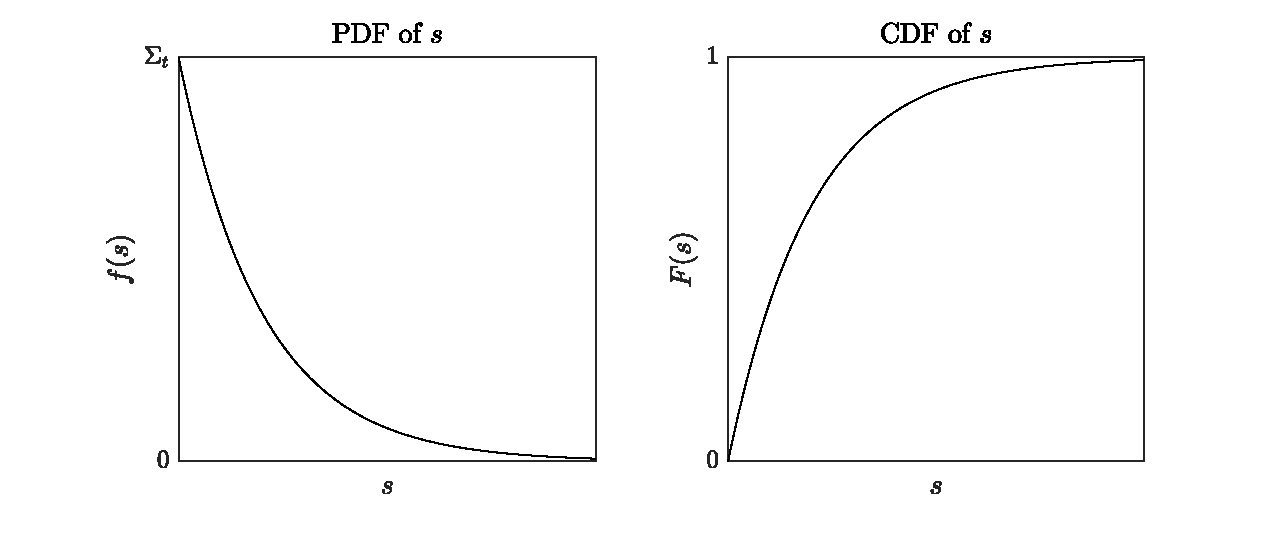
\includegraphics[scale=0.75]{images/cdf_pdf}
  \caption{Plots of the \acrshort{cdf} and \acrshort{pdf} for collision probability per distance travelled $s$.}
  \label{fig:cdf_pdf}
\end{figure}

As the \gls{cdf} ranges from zero to unity, we can sample its value by
a uniformly distributed random variable $\xi \in [0,1)$. The distance
traveled $s$, referred to as the path length, can then be expressed as
a function of this sampled random variable:
\begin{align*}
  F(s) = 1 - e^{-s\Sigma_t} &= \xi \\
  \ln(e^{-s \Sigma_t}) &= \ln(1-\xi) \\
  -\Sigma_t s &= \ln(\xi) \\
  s(\xi) &= \frac{1}{\Sigma_t}\ln(\xi)
\end{align*}

After sampling the path length of the neutron, its position is
updated, based on its original position and direction. We assumed that
the cross-section $\Sigma_t$ was constant in a material region, so the
sampled path length is only valid as long as the neutron remains in
that region.  If the neutron reaches the boundary between two material
regions, a new path length must be sampled using the cross-section of
the region it is entering. Each time a path length is sampled, the
distance to the nearest boundary in the direction of motion is
determined, and the neutron is moved to the boundary and path length
is resampled if appropriate. This can become computationally expensive
in complicated geometries and when the probability of crossing
boundaries with each sample path length is high.

\section{Woodcock Delta-tracking}
\label{sec:delta-tracking}

As discussed in Section~\ref{sec:ray_tracing}, the value of $\Sigma_t$
at a given position depends on the material at that point. Therefore,
$\Sigma_t(\vec{r})$ is a piece-wise discontinuous function that varies
arbitrarily with position and the geometry of the
problem~\cite{leppanen2013}. Using the ray tracing method, neutrons
must stop at boundaries to sample a new path length in a new material
region. To avoid the computational inefficiency that arises in
geometrically complicated regions, a rejection sampling technique
known as Woodcock delta-tracking was developed~\cite{woodcock1965}.

Woodcock delta-tracking introduces the concept of the majorant
cross-section, chosen to be the maximum of all material total
cross-sections in the region of interest.
\begin{equation}
  \label{eq:majorant}
  \Sigma_\mathrm{maj} \equiv \max_{\mathbf{r} \in \mathbb{V}}\{\Sigma_t(\mathbf{r})\}
\end{equation}
Where $\mathbb{V}$ is the volume of interest, as shown in a
one-dimensional region in Fig.~\ref{fig:sigma_maj}.
\begin{figure}[hbt]
  \centering
  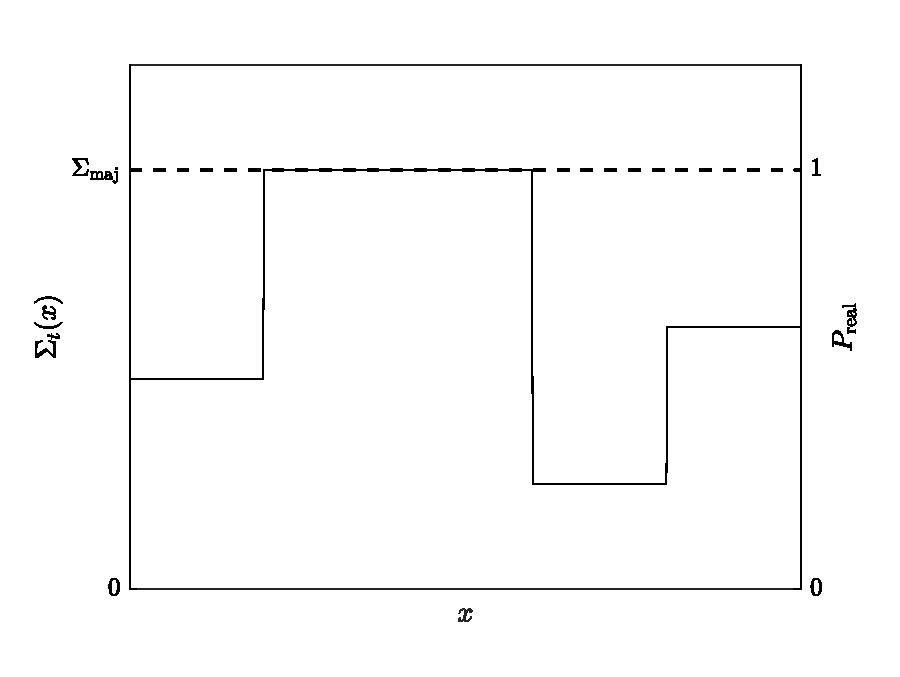
\includegraphics[scale=0.75]{images/sigma_maj}
  \caption{Total cross-section as a function of position in one
    dimension. The majorant cross-section is the largest value in the
    region of interest and determines the probability of a real collision.}
  \label{fig:sigma_maj}
\end{figure}

The majorant
cross-section can also be represented as the summation of the total
cross-section and a delta cross-section:
\begin{equation}
  \label{eq:majorant2}
  \Sigma_\mathrm{maj} = \Sigma_\delta(\mathbf{r}) +
  \Sigma_t(\mathbf{r}), \quad\forall \vec{r} \in \mathbb{V}
\end{equation}
Following from the definition of $\Sigma_\mathrm{maj}$ in
Eq.~\eqref{eq:majorant}, the function $\Sigma_\delta(\mathbf{r})$ is
chosen such that $\Sigma_\mathrm{maj}$ is constant for the entire
region of interest. At the position \textbf{r} where the maximum value
of $\Sigma_t(\mathbf{r})$ occurs, the delta cross-section is zero.

The majorant cross-section is constant throughout the entire region of
interest, so we can treat it as a single material. Following the same derivation in
Section~\ref{sec:ray_tracing}, the \gls{pdf} of the first collision occurring after
$s$ in the region of interest using the majorant cross-section is given by:
\begin{align}
  \label{eq:majorantpdf}
  f_\mathrm{maj}(s) &= \Sigma_\mathrm{maj}e^{-\Sigma_\mathrm{maj}s} \\
  & = (\Sigma_\delta(\mathbf{r}) +
    \Sigma_t(\mathbf{r}))e^{-\Sigma_\mathrm{maj}s}
\end{align}

In most of the region of interest, the majorant cross-section is not
the real cross-section. We must use a technique called rejection
sampling to simulate sampling the real $\Sigma_t(\vec{r})$ while
actually sampling using $\Sigma_\mathrm{maj}$. 

\subsubsection{Rejection Sampling}
\label{sec:rejection_sampling}
As described by Lux and
Koblinger~\cite{lux1991}, rejection sampling requires a \gls{pdf} of
interest, $f(x)$, and a second \gls{pdf} $g(x)$ for which:
\begin{equation}
  \label{eq:Mleq}
  f(x) \leq M\cdot g(x), \forall x
\end{equation} where $M \in \mathbb{R}$ is a constant.
Sampling from $M\cdot g(x)$ and accepting these samples with probability:
\begin{equation}
  \label{eq:preal}
  P = \frac{f(x)}{M\cdot g(x)}
\end{equation}
replicates sampling directly from $f(x)$. 

For example, consider a
\gls{pdf} of interest $f(x) = x^2$ on the interval $x \in (0,1]$ as shown
in Fig.~\ref{fig:circle_square}.
\begin{figure}[hbt]
  \centering
  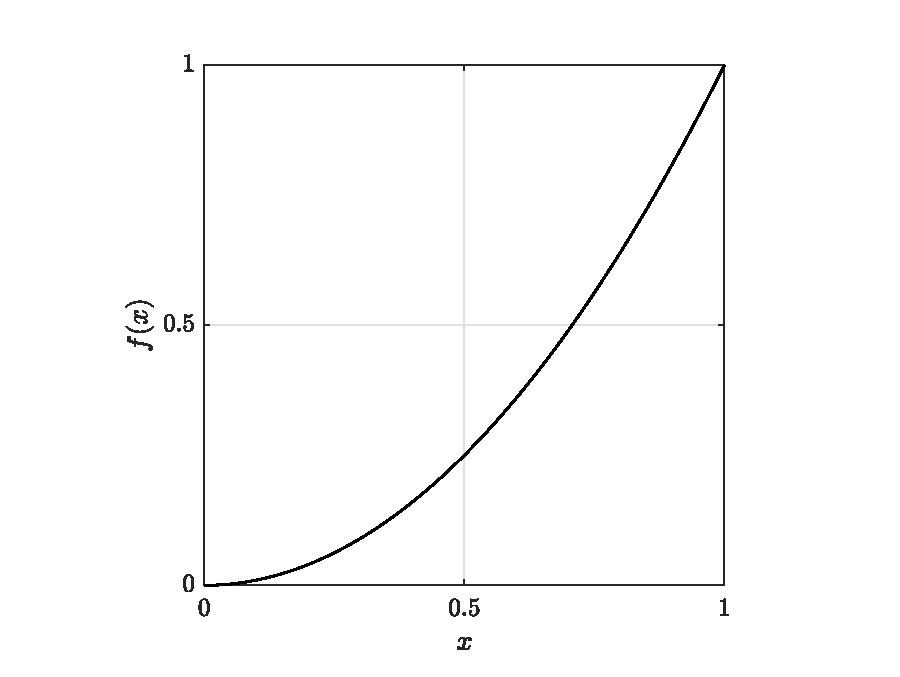
\includegraphics[scale=0.75]{images/circle}
  \caption{Example \acrshort{pdf} function $f(x)$.}
  \label{fig:circle_square}
\end{figure}
As described in the previous section, we could sample $f(x)$ using the
\gls{cdf} $F(x)$ found by integrating and then inverting. Instead, we can sample from a
different \gls{pdf} that is always majorant of $f(x)$, as defined in
Eq.~\eqref{eq:Mleq}. We can choose $g(x) = 1$, as $f(x) \leq 1$ on
the interval of interest. The \gls{cdf} of $g(x)$ is easy to
determine, because it is a constant value, and is just $G(x) =
x$. Therefore, we can sample $g(x)$ by simply sampling a random value $\xi
\in (0,1]$ and taking this as the value of $x$. To replicate sampling
from $f(x)$, we then sample another random value $\xi_2 \in (0,1]$ and
accept our value of $x$ using the probability defined in Eq.~\eqref{eq:preal}:
\begin{equation*}
  \xi_2 \leq \frac{f(x)}{g(x)} = x^2
\end{equation*}

\begin{minipage}{1.0\linewidth}
Following this algorithm using the simple Matlab script:
\begin{lstlisting}
a = [];                     % Accepted samples
for i = 1:1000
    x = rand;               % Sample g(x)
    y = rand;               % Gen random number xi2
    if y <= x.^2            % If xi2 <= f(x)/g(x)
        a(end+1) = x;       % Accept sample
    end
end
\end{lstlisting}
\end{minipage}

Generates the histogram shown in Fig.~\ref{fig:pdf_histogram}. As
expected, the procedure has reproduced the desired \gls{pdf} of $f(x)
= x^2$. Although this requires sampling two random variables, it can be
advantageous if $F(x)$ is difficult or impossible to invert.
\begin{figure}[hbtp]
  \centering
  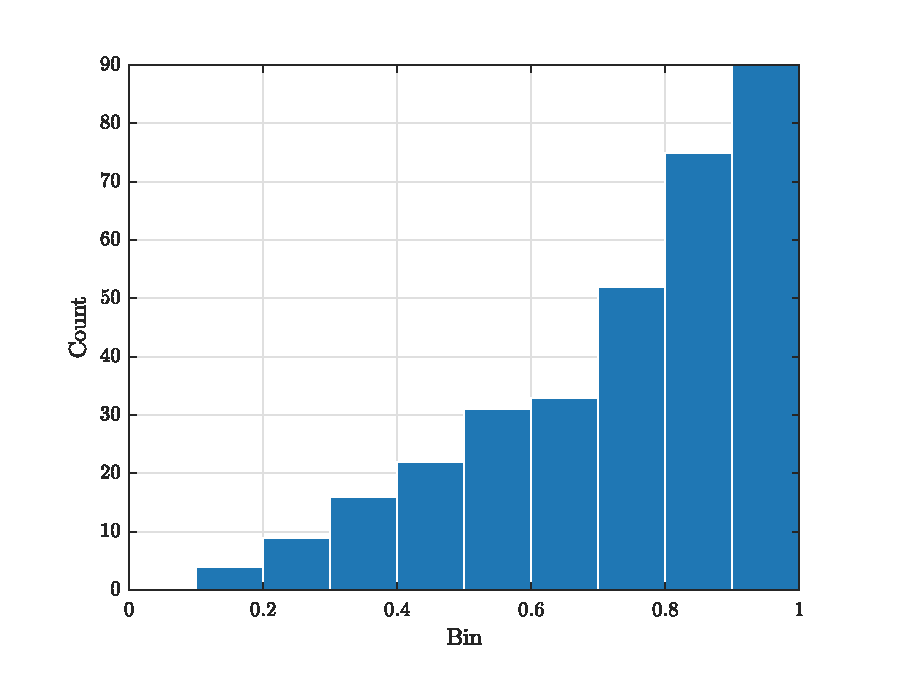
\includegraphics[scale=0.75]{images/pdf_histogram}
  \caption{Histogram of results from sampling and applying the
    rejection sampling algorithm.}
  \label{fig:pdf_histogram}
\end{figure}
\subsubsection{Application to Delta-tracking}
\label{sec:application_to_delta-tracking}

As we saw in Fig.~\ref{fig:sigma_maj}, the total cross-section
$\Sigma_t$ is a piecewise discontinuous function that depends on the
geometry of our problem. Therefore, each region has a different
\gls{cdf} for sampling path length, and described in
Section~\ref{sec:ray_tracing}. Using rejection sampling, we can sample
the real collision \gls{pdf}, using a different, simpler \gls{pdf}.
In Woodcock delta tracking, the second \gls{pdf} $g(x)$ is chosen to
be the majorant \gls{pdf}, Eq.~\eqref{eq:majorantpdf}. This is
beneficial because the majorant cross-section is constant over the
entire region.

These functions are both maximized at $x=0$, where the inequality of
Eq.~\eqref{eq:Mleq} is satisfied by setting $M=1$:
\begin{equation}
  \label{eq:cseq}
  \Sigma_t(\mathbf{r}) \leq \Sigma_\mathrm{maj}(\mathbf{r}), \forall
  \mathbf{r} \in \mathbb{V}
\end{equation}
We sample path length using the constant majorant
cross-section:
\begin{equation}
  \label{eq:majorantsample}
  s_\mathrm{maj}(\xi) = -\frac{1}{\Sigma_\mathrm{maj}}\ln(\xi)
\end{equation}
Which samples the \gls{pdf} defined in Eq.\eqref{eq:majorant}:
\begin{align*}
    f_\mathrm{maj}(s) &= \Sigma_\mathrm{maj}e^{-\Sigma_\mathrm{maj}s} \\
  & = (\Sigma_\delta(\mathbf{r}) +
    \Sigma_t(\mathbf{r}))e^{-\Sigma_\mathrm{maj}s}
\end{align*}
We can see that this \gls{pdf} is the sum of two different ones: one
representing actual collisions based on the real total cross-section
$\Sigma_t$ and one representing the non-physical collisions based on
$\Sigma_\delta$. We call these non-physical collisions ``virtual''
collisions, and these should be eliminated by our rejection
sampling. To apply rejection sampling, we therefore pick the \gls{pdf}
we want to sample $f(x)$ and the \gls{pdf} we will actually sample
$g(x)$ as such:
\begin{align*}
  f(x) &= \Sigma_t(\vec{r})e^{-\Sigma_\mathrm{maj}s} \\
  g(x) &= \Sigma_\mathrm{maj}e^{-\Sigma_\mathrm{maj}s}
\end{align*}
We will therefore accept samples with the probability given
in Eq.~\eqref{eq:preal}:
\begin{align}
  \label{eq:prealfinal}
  P_{\mathrm{real}}(\vec{r}) &= \frac{f(x)}{Mg(x)} =
      \frac{\Sigma_t(\mathbf{r})e^{-\Sigma_\mathrm{maj}s}}{\Sigma_\mathrm{maj}e^{-\Sigma_\mathrm{maj}s}}
  = \frac{\Sigma_t(\mathbf{r})}{\Sigma_\mathrm{maj}}
\end{align}
We will refer to this as the probability of a ``real'' collision,
$P_\mathrm{real}$ to differentiate these physical collisions from the
non-physical virtual collisions. It is important to note that the
probability is independent of path length $s$, but is dependent on
position $\vec{r}$. At each collision, the material region at the
neutron position must be determined, but we do not need to explicitly
track boundaries nor calculate their distance each time a path length
is sampled. The algorithm for delta-tracking is shown in
Fig.~\ref{fig:dt}.

\begin{figure}[p]
  \centering
  \begin{algorithm}[H]
\caption{Delta-tracking}\label{alg:dt}
\begin{algorithmic}[1]
  \State \textbf{Sample} path length

  \State \textbf{Look up} location to get $\Sigma_t(\vec{r})$
  \State $P_\mathrm{real} \gets
  \frac{\Sigma_t(\vec{r})}{\Sigma_\mathrm{maj}}$
  \State \textbf{Sample} random number $\xi \in [0,1)$
  \If{$\xi < P_\mathrm{real}$} \Comment{Collision is real}
  \State \textbf{Execute} real collision
    \Else \Comment{Collision is virtual}
    \State \textbf{Execute} virtual collision
  \EndIf
\end{algorithmic}
\end{algorithm}
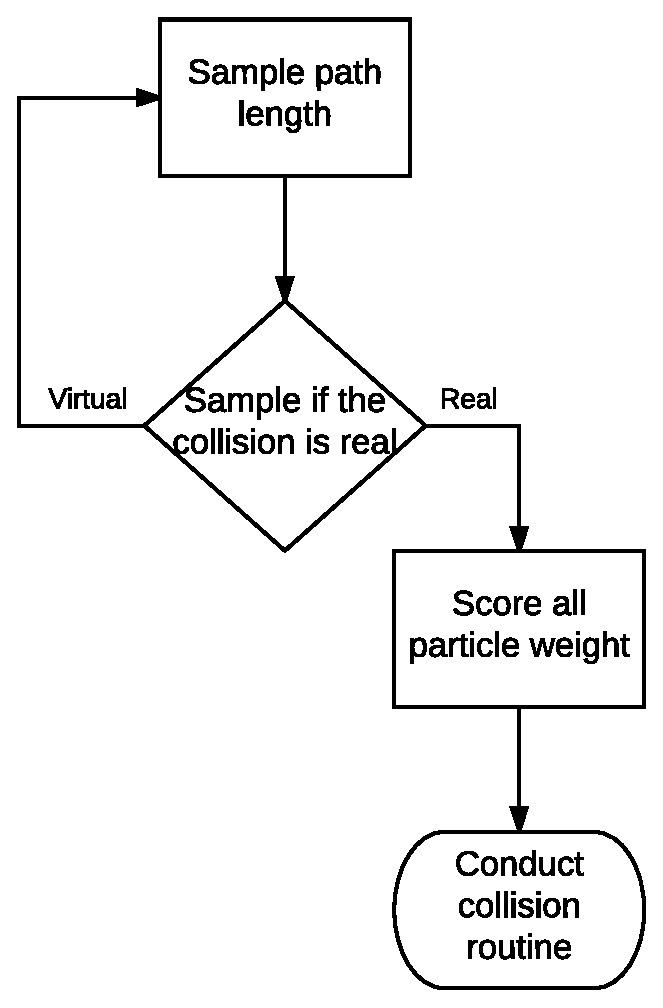
\includegraphics[scale=0.5]{images/dt}
  \caption{Delta-tracking algorithm and flow chart.}
  \label{fig:dt}
\end{figure}

Now, the path length can be sampled across multiple material regions
of varying $\Sigma_t$ without explicitly stopping the neutron at a
given boundary. This method can become computationally inefficient in
regions where the total cross-section is much less than the majorant
cross-section, leading to oversampling of virtual collisions. This is
seen in geometries that include localized absorbers, such as control
rods. Another downside is that the \gls{tle} for
flux cannot be used. The \gls{tle} requires calculating the track-lengths
within a particular material cell, and therefore does not work when
the neutron path length can cross one or more material
boundaries. The \gls{cfe} can be used in its
place, but often results in inferior statistics as not every track
length sampled ends in a collision~\cite{leppanen2013}.

\section{The Serpent 2 Monte Carlo Code}
\label{sec:serpent2}

The Serpent Monte Carlo code was developed at \gls{vtt} as a PhD
thesis project~\cite{leppanen2007}. A second iteration of the code
Serpent 2, is currently under development. The Serpent and Serpent 2
Monte Carlo Code use a combination of surface tracking, Woodcock
delta-tracking, and rejection sampling for non-uniform density
distributions. Serpent 2 selects between surface tracking and
delta-tracking by examining the ratio of total cross-section to
majorant cross-section~\cite{leppanen2010}. In regions where many
virtual collisions would occur, the code preferentially switches to
ray tracing. This is to avoid the computational inefficiency of
processing virtual collisions that provide no statistics. This
selection determined by a constant $c$ and the inequality in
Eq.~\eqref{eq:s2deltasurface}.
\begin{equation}
  \label{eq:s2deltasurface}
  \frac{\Sigma_t(\vec{r})}{\Sigma_\mathrm{maj}} > 1 - c
\end{equation}
If this inequality is true, delta-tracking is used, otherwise
ray-tracing (referred to as surface-tracking in Serpent 2) is used. By
default, the value of $c$ is 0.9, as this was determined to produce
the best improvement in run time~\cite{leppanen2010}. We note that
this inequality is identical to the value of $P_\mathrm{real}$, and
this scheme is summarized in Fig.~\ref{fig:ray_wdt_normal}.  Prior to
sampling path length, the code tests this ratio for the current
neutron position and determines if surface tracking or delta-tracking
should be used. If delta-tracking is used, the code then determines if
the collision is virtual or real. The value of $c$ can be set in the
input file using \verb|set dt|.
\begin{figure}[hbtp]\centering
  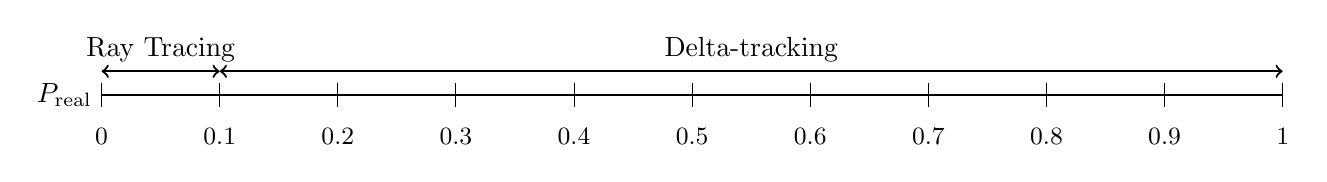
\begin{tikzpicture}[scale=1.5]
    \draw[thick] (0,0) -- (10.0,0);
    \foreach \x in {0,1,...,10}
    {
      \draw (\x, 0.1) -- (\x, -0.1);
      \pgfmathsetmacro\result{\x * 0.1}
      \node [below] at (\x, -0.2) {\small $\pgfmathprintnumber{\result}$};
    }
    \node [left] at (0,0) {$P_{\mathrm{real}}$};
    \draw[ thick, <->] (0,0.2) -- (1,0.2);
    \draw[ thick, <->] (1,0.2) -- (10,0.2);
    \node [above] at (0.5, 0.2) {Ray Tracing};
    \node [above] at (5.5, 0.2) {Delta-tracking};
  \end{tikzpicture}
  \caption{Ray-tracing and delta-tracking threshold values in
    standard Serpent 2.}
  \label{fig:ray_wdt_normal}
\end{figure}

\subsubsection{Nonuniform Density Distributions}
\label{sec:nonuniform}

Rejection sampling can also be used when the total cross-section is
not constant within a material region. As discussed by
Lepp\"{a}nen~\cite{leppanen2013}, Serpent 2 conducts a rejection
sampling routine similar to Woodcock delta-tracking in these
regions. Instead of sampling from a majorant cross-section across
multiple materials, a maximum cross-section for the single material
region is used. Unlike delta-tracking, this requires stopping the
neutron at boundaries and resampling path lengths. This algorithm is
not modified by the implementation of \gls{wdt} and none of the input
files used to assess \gls{wdt} use this feature.


%%% Local Variables:
%%% mode: latex
%%% TeX-master: "../masters_report"
%%% End:
